\documentclass[a4paper, 12pt]{article}
%%%%%%%%%%%%%%%%%%%%%%%%%%%%%%%%%%%%%%%%%%%%%%%%%%%%%%%%%%%%%%%%%%%%%%%%%%%%%%%
%                                Basic Packages                               %
%%%%%%%%%%%%%%%%%%%%%%%%%%%%%%%%%%%%%%%%%%%%%%%%%%%%%%%%%%%%%%%%%%%%%%%%%%%%%%%

% Gives us multiple colors.
\usepackage[usenames,dvipsnames,pdftex]{xcolor}
% Lets us style link colors.
\usepackage{hyperref}
% Lets us import images and graphics.
\usepackage{graphicx}
% Lets us use figures in floating environments.
\usepackage{float}
% Lets us create multiple columns.
\usepackage{multicol}
% Gives us better math syntax.
\usepackage{amsmath,amsfonts,mathtools,amsthm,amssymb}
% Lets us strikethrough text.
\usepackage{cancel}
% Lets us edit the caption of a figure.
\usepackage{caption}
% Lets us import pdf directly in our tex code.
\usepackage{pdfpages}
% Lets us do algorithm stuff.
\usepackage[ruled,vlined,linesnumbered]{algorithm2e}
% Use a smiley face for our qed symbol.
\usepackage{tikzsymbols}
% \usepackage{fullpage} %%smaller margins
\usepackage[shortlabels]{enumitem}

\setlist[enumerate]{font={\bfseries}} % global settings, for all lists

\usepackage{setspace}
\usepackage[margin=1in, headsep=12pt]{geometry}
\usepackage{wrapfig}
\usepackage{listings}
\usepackage{parskip}

\definecolor{codegreen}{rgb}{0,0.6,0}
\definecolor{codegray}{rgb}{0.5,0.5,0.5}
\definecolor{codepurple}{rgb}{0.58,0,0.82}
\definecolor{backcolour}{rgb}{0.95,0.95,0.95}

\lstdefinestyle{mystyle}{
    backgroundcolor=\color{backcolour},   
    commentstyle=\color{codegreen},
    keywordstyle=\color{magenta},
    numberstyle=\tiny\color{codegray},
    stringstyle=\color{codepurple},
    basicstyle=\ttfamily\footnotesize,
    breakatwhitespace=false,         
    breaklines=true,                 
    captionpos=b,                    
    keepspaces=true,                 
    numbers=left,                    
    numbersep=5pt,                  
    showspaces=false,                
    showstringspaces=false,
    showtabs=false,                  
    tabsize=2,
    numbers=none
}

\lstset{style=mystyle}
\def\class{article}


%%%%%%%%%%%%%%%%%%%%%%%%%%%%%%%%%%%%%%%%%%%%%%%%%%%%%%%%%%%%%%%%%%%%%%%%%%%%%%%
%                                Basic Settings                               %
%%%%%%%%%%%%%%%%%%%%%%%%%%%%%%%%%%%%%%%%%%%%%%%%%%%%%%%%%%%%%%%%%%%%%%%%%%%%%%%

%%%%%%%%%%%%%
%  Symbols  %
%%%%%%%%%%%%%

\let\implies\Rightarrow
\let\impliedby\Leftarrow
\let\iff\Leftrightarrow
\let\epsilon\varepsilon
%%%%%%%%%%%%
%  Tables  %
%%%%%%%%%%%%

\setlength{\tabcolsep}{5pt}
\renewcommand\arraystretch{1.5}

%%%%%%%%%%%%%%
%  SI Unitx  %
%%%%%%%%%%%%%%

\usepackage{siunitx}
\sisetup{locale = FR}

%%%%%%%%%%
%  TikZ  %
%%%%%%%%%%

\usepackage[framemethod=TikZ]{mdframed}
\usepackage{tikz}
\usepackage{tikz-cd}
\usepackage{tikzsymbols}

\usetikzlibrary{intersections, angles, quotes, calc, positioning}
\usetikzlibrary{arrows.meta}

\tikzset{
    force/.style={thick, {Circle[length=2pt]}-stealth, shorten <=-1pt}
}

%%%%%%%%%%%%%%%
%  PGF Plots  %
%%%%%%%%%%%%%%%

\usepackage{pgfplots}
\pgfplotsset{width=10cm, compat=newest}

%%%%%%%%%%%%%%%%%%%%%%%
%  Center Title Page  %
%%%%%%%%%%%%%%%%%%%%%%%

\usepackage{titling}
\renewcommand\maketitlehooka{\null\mbox{}\vfill}
\renewcommand\maketitlehookd{\vfill\null}

%%%%%%%%%%%%%%%%%%%%%%%%%%%%%%%%%%%%%%%%%%%%%%%%%%%%%%%
%  Create a grey background in the middle of the PDF  %
%%%%%%%%%%%%%%%%%%%%%%%%%%%%%%%%%%%%%%%%%%%%%%%%%%%%%%%

\usepackage{eso-pic}
\newcommand\definegraybackground{
    \definecolor{reallylightgray}{HTML}{FAFAFA}
    \AddToShipoutPicture{
        \ifthenelse{\isodd{\thepage}}{
            \AtPageLowerLeft{
                \put(\LenToUnit{\dimexpr\paperwidth-222pt},0){
                    \color{reallylightgray}\rule{222pt}{297mm}
                }
            }
        }
        {
            \AtPageLowerLeft{
                \color{reallylightgray}\rule{222pt}{297mm}
            }
        }
    }
}

%%%%%%%%%%%%%%%%%%%%%%%%
%  Modify Links Color  %
%%%%%%%%%%%%%%%%%%%%%%%%

\hypersetup{
    % Enable highlighting links.
    colorlinks,
    % Change the color of links to blue.
    urlcolor=blue,
    % Change the color of citations to black.
    citecolor={black},
    % Change the color of url's to blue with some black.
    linkcolor={blue!80!black}
}

%%%%%%%%%%%%%%%%%%
% Fix WrapFigure %
%%%%%%%%%%%%%%%%%%

\newcommand{\wrapfill}{\par\ifnum\value{WF@wrappedlines}>0
        \parskip=0pt
        \addtocounter{WF@wrappedlines}{-1}%
        \null\vspace{\arabic{WF@wrappedlines}\baselineskip}%
        \WFclear
    \fi}

%%%%%%%%%%%%%%%%%
% Multi Columns %
%%%%%%%%%%%%%%%%%

\let\multicolmulticols\multicols
\let\endmulticolmulticols\endmulticols

\RenewDocumentEnvironment{multicols}{mO{}}
{%
    \ifnum#1=1
        #2%
    \else % More than 1 column
        \multicolmulticols{#1}[#2]
    \fi
}
{%
    \ifnum#1=1
    \else % More than 1 column
        \endmulticolmulticols
    \fi
}

\newlength{\thickarrayrulewidth}
\setlength{\thickarrayrulewidth}{5\arrayrulewidth}


%%%%%%%%%%%%%%%%%%%%%%%%%%%%%%%%%%%%%%%%%%%%%%%%%%%%%%%%%%%%%%%%%%%%%%%%%%%%%%%
%                           School Specific Commands                          %
%%%%%%%%%%%%%%%%%%%%%%%%%%%%%%%%%%%%%%%%%%%%%%%%%%%%%%%%%%%%%%%%%%%%%%%%%%%%%%%

%%%%%%%%%%%%%%%%%%%%%%%%%%%
%  Initiate New Counters  %
%%%%%%%%%%%%%%%%%%%%%%%%%%%

\newcounter{lecturecounter}

%%%%%%%%%%%%%%%%%%%%%%%%%%
%  Helpful New Commands  %
%%%%%%%%%%%%%%%%%%%%%%%%%%

\makeatletter

\newcommand\resetcounters{
    % Reset the counters for subsection, subsubsection and the definition
    % all the custom environments.
    \setcounter{subsection}{0}
    \setcounter{subsubsection}{0}
    \setcounter{definition0}{0}
    \setcounter{paragraph}{0}
    \setcounter{theorem}{0}
    \setcounter{claim}{0}
    \setcounter{corollary}{0}
    \setcounter{proposition}{0}
    \setcounter{lemma}{0}
    \setcounter{exercise}{0}
    \setcounter{problem}{0}
    
    \setcounter{subparagraph}{0}
    % \@ifclasswith\class{nocolor}{
    %     \setcounter{definition}{0}
    % }{}
}

%%%%%%%%%%%%%%%%%%%%%
%  Lecture Command  %
%%%%%%%%%%%%%%%%%%%%%

\usepackage{xifthen}

% EXAMPLE:
% 1. \lecture{Oct 17 2022 Mon (08:46:48)}{Lecture Title}
% 2. \lecture[4]{Oct 17 2022 Mon (08:46:48)}{Lecture Title}
% 3. \lecture{Oct 17 2022 Mon (08:46:48)}{}
% 4. \lecture[4]{Oct 17 2022 Mon (08:46:48)}{}
% Parameters:
% 1. (Optional) lecture number.
% 2. Time and date of lecture.
% 3. Lecture Title.
\def\@lecture{}
\def\@lectitle{}
\def\@leccount{}
\newcommand\lecture[3]{
    \newpage

    % Check if user passed the lecture title or not.
    \def\@leccount{Lecture #1}
    \ifthenelse{\isempty{#3}}{
        \def\@lecture{Lecture #1}
        \def\@lectitle{Lecture #1}
    }{
        \def\@lecture{Lecture #1: #3}
        \def\@lectitle{#3}
    }

    \setcounter{section}{#1}
    \renewcommand\thesubsection{#1.\arabic{subsection}}
    
    \phantomsection
    \addcontentsline{toc}{section}{\@lecture}
    \resetcounters

    \begin{mdframed}
        \begin{center}
            \Large \textbf{\@leccount}
            
            \vspace*{0.2cm}
            
            \large \@lectitle
            
            
            \vspace*{0.2cm}

            \normalsize #2
        \end{center}
    \end{mdframed}

}

%%%%%%%%%%%%%%%%%%%%
%  Import Figures  %
%%%%%%%%%%%%%%%%%%%%

\usepackage{import}
\pdfminorversion=7

% EXAMPLE:
% 1. \incfig{limit-graph}
% 2. \incfig[0.4]{limit-graph}
% Parameters:
% 1. The figure name. It should be located in figures/NAME.tex_pdf.
% 2. (Optional) The width of the figure. Example: 0.5, 0.35.
\newcommand\incfig[2][1]{%
    \def\svgwidth{#1\columnwidth}
    \import{./figures/}{#2.pdf_tex}
}

\begingroup\expandafter\expandafter\expandafter\endgroup
\expandafter\ifx\csname pdfsuppresswarningpagegroup\endcsname\relax
\else
    \pdfsuppresswarningpagegroup=1\relax
\fi

%%%%%%%%%%%%%%%%%
% Fancy Headers %
%%%%%%%%%%%%%%%%%

\usepackage{fancyhdr}

% Force a new page.
\newcommand\forcenewpage{\clearpage\mbox{~}\clearpage\newpage}

% This command makes it easier to manage my headers and footers.
\newcommand\createintro{
    % Use roman page numbers (e.g. i, v, vi, x, ...)
    \pagenumbering{roman}

    % Display the page style.
    \maketitle
    % Make the title pagestyle empty, meaning no fancy headers and footers.
    \thispagestyle{empty}
    % Create a newpage.
    \newpage

    % Input the intro.tex page if it exists.
    \IfFileExists{intro.tex}{ % If the intro.tex file exists.
        % Input the intro.tex file.
        \textbf{Course}: MATH 16300: Honors Calculus III

\textbf{Section}: 43

\textbf{Professor}: Minjae Park

\textbf{At}: The University of Chicago

\textbf{Quarter}: Spring 2023

\textbf{Course materials}: Calculus by Spivak (4th Edition), Calculus On Manifolds by Spivak

\vspace{1cm}
\textbf{Disclaimer}: This document will inevitably contain some mistakes, both simple typos and serious logical and mathematical errors. Take what you read with a grain of salt as it is made by an undergraduate student going through the learning process himself. If you do find any error, I would really appreciate it if you can let me know by email at \href{mailto:conghungletran@gmail.com}{conghungletran@gmail.com}.

        % Make the pagestyle fancy for the intro.tex page.
        \pagestyle{fancy}

        % Remove the line for the header.
        \renewcommand\headrulewidth{0pt}

        % Remove all header stuff.
        \fancyhead{}

        % Add stuff for the footer in the center.
        % \fancyfoot[C]{
        %   \textit{For more notes like this, visit
        %   \href{\linktootherpages}{\shortlinkname}}. \\
        %   \vspace{0.1cm}
        %   \hrule
        %   \vspace{0.1cm}
        %   \@author, \\
        %   \term: \academicyear, \\
        %   Last Update: \@date, \\
        %   \faculty
        % }

        \newpage
    }{ % If the intro.tex file doesn't exist.
        % Force a \newpageage.
        % \forcenewpage
        \newpage
    }

    % Remove the center stuff we did above, and replace it with just the page
    % number, which is still in roman numerals.
    \fancyfoot[C]{\thepage}
    % Add the table of contents.
    \tableofcontents
    % Force a new page.
    \newpage

    % Move the page numberings back to arabic, from roman numerals.
    \pagenumbering{arabic}
    % Set the page number to 1.
    \setcounter{page}{1}

    % Add the header line back.
    \renewcommand\headrulewidth{0.4pt}
    % In the top right, add the lecture title.
    \fancyhead[R]{\footnotesize \@lecture}
    % In the top left, add the author name.
    \fancyhead[L]{\footnotesize \@author}
    % In the bottom center, add the page.
    \fancyfoot[C]{\thepage}
    % Add a nice gray background in the middle of all the upcoming pages.
    % \definegraybackground
}

\makeatother


%%%%%%%%%%%%%%%%%%%%%%%%%%%%%%%%%%%%%%%%%%%%%%%%%%%%%%%%%%%%%%%%%%%%%%%%%%%%%%%
%                               Custom Commands                               %
%%%%%%%%%%%%%%%%%%%%%%%%%%%%%%%%%%%%%%%%%%%%%%%%%%%%%%%%%%%%%%%%%%%%%%%%%%%%%%%

%%%%%%%%%%%%
%  Circle  %
%%%%%%%%%%%%

\newcommand*\circled[1]{\tikz[baseline= (char.base)]{
        \node[shape=circle,draw,inner sep=1pt] (char) {#1};}
}

%%%%%%%%%%%%%%%%%%%
%  Todo Commands  %
%%%%%%%%%%%%%%%%%%%

% \usepackage{xargs}
% \usepackage[colorinlistoftodos]{todonotes}

% \makeatletter

% \@ifclasswith\class{working}{
%     \newcommandx\unsure[2][1=]{\todo[linecolor=red,backgroundcolor=red!25,bordercolor=red,#1]{#2}}
%     \newcommandx\change[2][1=]{\todo[linecolor=blue,backgroundcolor=blue!25,bordercolor=blue,#1]{#2}}
%     \newcommandx\info[2][1=]{\todo[linecolor=OliveGreen,backgroundcolor=OliveGreen!25,bordercolor=OliveGreen,#1]{#2}}
%     \newcommandx\improvement[2][1=]{\todo[linecolor=Plum,backgroundcolor=Plum!25,bordercolor=Plum,#1]{#2}}

%     \newcommand\listnotes{
%         \newpage
%         \listoftodos[Notes]
%     }
% }{
%     \newcommandx\unsure[2][1=]{}
%     \newcommandx\change[2][1=]{}
%     \newcommandx\info[2][1=]{}
%     \newcommandx\improvement[2][1=]{}

%     \newcommand\listnotes{}
% }

% \makeatother

%%%%%%%%%%%%%
%  Correct  %
%%%%%%%%%%%%%

% EXAMPLE:
% 1. \correct{INCORRECT}{CORRECT}
% Parameters:
% 1. The incorrect statement.
% 2. The correct statement.
\definecolor{correct}{HTML}{009900}
\newcommand\correct[2]{{\color{red}{#1 }}\ensuremath{\to}{\color{correct}{ #2}}}


%%%%%%%%%%%%%%%%%%%%%%%%%%%%%%%%%%%%%%%%%%%%%%%%%%%%%%%%%%%%%%%%%%%%%%%%%%%%%%%
%                                 Environments                                %
%%%%%%%%%%%%%%%%%%%%%%%%%%%%%%%%%%%%%%%%%%%%%%%%%%%%%%%%%%%%%%%%%%%%%%%%%%%%%%%

\usepackage{varwidth}
\usepackage{thmtools}
\usepackage[most,many,breakable]{tcolorbox}

\tcbuselibrary{theorems,skins,hooks}
\usetikzlibrary{arrows,calc,shadows.blur}

%%%%%%%%%%%%%%%%%%%
%  Define Colors  %
%%%%%%%%%%%%%%%%%%%

% color prototype
% \definecolor{color}{RGB}{45, 111, 177}

% ESSENTIALS: 
\definecolor{myred}{HTML}{c74540}
\definecolor{myblue}{HTML}{072b85}
\definecolor{mygreen}{HTML}{388c46}
\definecolor{myblack}{HTML}{000000}

\colorlet{definition_color}{myred}

\colorlet{theorem_color}{myblue}
\colorlet{lemma_color}{myblue}
\colorlet{prop_color}{myblue}
\colorlet{corollary_color}{myblue}
\colorlet{claim_color}{myblue}

\colorlet{proof_color}{myblack}
\colorlet{example_color}{myblack}
\colorlet{exercise_color}{myblack}

% MISCS: 
%%%%%%%%%%%%%%%%%%%%%%%%%%%%%%%%%%%%%%%%%%%%%%%%%%%%%%%%%
%  Create Environments Styles Based on Given Parameter  %
%%%%%%%%%%%%%%%%%%%%%%%%%%%%%%%%%%%%%%%%%%%%%%%%%%%%%%%%%

% \mdfsetup{skipabove=1em,skipbelow=0em}

%%%%%%%%%%%%%%%%%%%%%%
%  Helpful Commands  %
%%%%%%%%%%%%%%%%%%%%%%

% EXAMPLE:
% 1. \createnewtheoremstyle{thmdefinitionbox}{}{}
% 2. \createnewtheoremstyle{thmtheorembox}{}{}
% 3. \createnewtheoremstyle{thmproofbox}{qed=\qedsymbol}{
%       rightline=false, topline=false, bottomline=false
%    }
% Parameters:
% 1. Theorem name.
% 2. Any extra parameters to pass directly to declaretheoremstyle.
% 3. Any extra parameters to pass directly to mdframed.
\newcommand\createnewtheoremstyle[3]{
    \declaretheoremstyle[
        headfont=\bfseries\sffamily, bodyfont=\normalfont, #2,
        mdframed={
                #3,
            },
    ]{#1}
}

% EXAMPLE:
% 1. \createnewcoloredtheoremstyle{thmdefinitionbox}{definition}{}{}
% 2. \createnewcoloredtheoremstyle{thmexamplebox}{example}{}{
%       rightline=true, leftline=true, topline=true, bottomline=true
%     }
% 3. \createnewcoloredtheoremstyle{thmproofbox}{proof}{qed=\qedsymbol}{backgroundcolor=white}
% Parameters:
% 1. Theorem name.
% 2. Color of theorem.
% 3. Any extra parameters to pass directly to declaretheoremstyle.
% 4. Any extra parameters to pass directly to mdframed.

% change backgroundcolor to #2!5 if user wants a colored backdrop to theorem environments. It's a cool color theme, but there's too much going on in the page.
\newcommand\createnewcoloredtheoremstyle[4]{
    \declaretheoremstyle[
        headfont=\bfseries\sffamily\color{#2},
        bodyfont=\normalfont,
        headpunct=,
        headformat = \NAME~\NUMBER\NOTE \hfill\smallskip\linebreak,
        #3,
        mdframed={
                outerlinewidth=0.75pt,
                rightline=false,
                leftline=false,
                topline=false,
                bottomline=false,
                backgroundcolor=white,
                skipabove = 5pt,
                skipbelow = 0pt,
                linecolor=#2,
                innertopmargin = 0pt,
                innerbottommargin = 0pt,
                innerrightmargin = 4pt,
                innerleftmargin= 6pt,
                leftmargin = -6pt,
                #4,
            },
    ]{#1}
}



%%%%%%%%%%%%%%%%%%%%%%%%%%%%%%%%%%%
%  Create the Environment Styles  %
%%%%%%%%%%%%%%%%%%%%%%%%%%%%%%%%%%%

\makeatletter
\@ifclasswith\class{nocolor}{
    % Environments without color.

    % ESSENTIALS:
    \createnewtheoremstyle{thmdefinitionbox}{}{}
    \createnewtheoremstyle{thmtheorembox}{}{}
    \createnewtheoremstyle{thmproofbox}{qed=\qedsymbol}{}
    \createnewtheoremstyle{thmcorollarybox}{}{}
    \createnewtheoremstyle{thmlemmabox}{}{}
    \createnewtheoremstyle{thmclaimbox}{}{}
    \createnewtheoremstyle{thmexamplebox}{}{}

    % MISCS: 
    \createnewtheoremstyle{thmpropbox}{}{}
    \createnewtheoremstyle{thmexercisebox}{}{}
    \createnewtheoremstyle{thmexplanationbox}{}{}
    \createnewtheoremstyle{thmremarkbox}{}{}
    
    % STYLIZED MORE BELOW
    \createnewtheoremstyle{thmquestionbox}{}{}
    \createnewtheoremstyle{thmsolutionbox}{qed=\qedsymbol}{}
}{
    % Environments with color.

    % ESSENTIALS: definition, theorem, proof, corollary, lemma, claim, example
    \createnewcoloredtheoremstyle{thmdefinitionbox}{definition_color}{}{leftline=false}
    \createnewcoloredtheoremstyle{thmtheorembox}{theorem_color}{}{leftline=false}
    \createnewcoloredtheoremstyle{thmproofbox}{proof_color}{qed=\qedsymbol}{}
    \createnewcoloredtheoremstyle{thmcorollarybox}{corollary_color}{}{leftline=false}
    \createnewcoloredtheoremstyle{thmlemmabox}{lemma_color}{}{leftline=false}
    \createnewcoloredtheoremstyle{thmpropbox}{prop_color}{}{leftline=false}
    \createnewcoloredtheoremstyle{thmclaimbox}{claim_color}{}{leftline=false}
    \createnewcoloredtheoremstyle{thmexamplebox}{example_color}{}{}
    \createnewcoloredtheoremstyle{thmexplanationbox}{example_color}{qed=\qedsymbol}{}
    \createnewcoloredtheoremstyle{thmremarkbox}{theorem_color}{}{}

    \createnewcoloredtheoremstyle{thmmiscbox}{black}{}{}

    \createnewcoloredtheoremstyle{thmexercisebox}{exercise_color}{}{}
    \createnewcoloredtheoremstyle{thmproblembox}{theorem_color}{}{leftline=false}
    \createnewcoloredtheoremstyle{thmsolutionbox}{mygreen}{qed=\qedsymbol}{}
}
\makeatother

%%%%%%%%%%%%%%%%%%%%%%%%%%%%%
%  Create the Environments  %
%%%%%%%%%%%%%%%%%%%%%%%%%%%%%
\declaretheorem[numberwithin=section, style=thmdefinitionbox,     name=Definition]{definition}
\declaretheorem[numberwithin=section, style=thmtheorembox,     name=Theorem]{theorem}
\declaretheorem[numbered=no,          style=thmexamplebox,     name=Example]{example}
\declaretheorem[numberwithin=section, style=thmtheorembox,       name=Claim]{claim}
\declaretheorem[numberwithin=section, style=thmcorollarybox,   name=Corollary]{corollary}
\declaretheorem[numberwithin=section, style=thmpropbox,        name=Proposition]{proposition}
\declaretheorem[numberwithin=section, style=thmlemmabox,       name=Lemma]{lemma}
\declaretheorem[numberwithin=section, style=thmexercisebox,    name=Exercise]{exercise}
\declaretheorem[numbered=no,          style=thmproofbox,       name=Proof]{proof0}
\declaretheorem[numbered=no,          style=thmexplanationbox, name=Explanation]{explanation}
\declaretheorem[numbered=no,          style=thmsolutionbox,    name=Solution]{solution}
\declaretheorem[numberwithin=section,          style=thmproblembox,     name=Problem]{problem}
\declaretheorem[numbered=no,          style=thmmiscbox,    name=Intuition]{intuition}
\declaretheorem[numbered=no,          style=thmmiscbox,    name=Goal]{goal}
\declaretheorem[numbered=no,          style=thmmiscbox,    name=Recall]{recall}
\declaretheorem[numbered=no,          style=thmmiscbox,    name=Motivation]{motivation}
\declaretheorem[numbered=no,          style=thmmiscbox,    name=Remark]{remark}
\declaretheorem[numbered=no,          style=thmmiscbox,    name=Observe]{observe}
\declaretheorem[numbered=no,          style=thmmiscbox,    name=Question]{question}


%%%%%%%%%%%%%%%%%%%%%%%%%%%%
%  Edit Proof Environment  %
%%%%%%%%%%%%%%%%%%%%%%%%%%%%

\renewenvironment{proof}[2][\proofname]{
    % \vspace{-12pt}
    \begin{proof0} [#2]
        }{\end{proof0}}

\theoremstyle{definition}

\newtheorem*{notation}{Notation}
\newtheorem*{previouslyseen}{As previously seen}
\newtheorem*{property}{Property}
% \newtheorem*{intuition}{Intuition}
% \newtheorem*{goal}{Goal}
% \newtheorem*{recall}{Recall}
% \newtheorem*{motivation}{Motivation}
% \newtheorem*{remark}{Remark}
% \newtheorem*{observe}{Observe}

\author{Hung C. Le Tran}


%%%% MATH SHORTHANDS %%%%
%% blackboard bold math capitals
\DeclareMathOperator*{\esssup}{ess\,sup}
\DeclareMathOperator*{\Hom}{Hom}
\newcommand{\bbf}{\mathbb{F}}
\newcommand{\bbn}{\mathbb{N}}
\newcommand{\bbq}{\mathbb{Q}}
\newcommand{\bbr}{\mathbb{R}}
\newcommand{\bbz}{\mathbb{Z}}
\newcommand{\bbc}{\mathbb{C}}
\newcommand{\bbk}{\mathbb{K}}
\newcommand{\bbm}{\mathbb{M}}
\newcommand{\bbp}{\mathbb{P}}
\newcommand{\bbe}{\mathbb{E}}

\newcommand{\bfw}{\mathbf{w}}
\newcommand{\bfx}{\mathbf{x}}
\newcommand{\bfX}{\mathbf{X}}
\newcommand{\bfy}{\mathbf{y}}
\newcommand{\bfyhat}{\mathbf{\hat{y}}}

\newcommand{\calb}{\mathcal{B}}
\newcommand{\calf}{\mathcal{F}}
\newcommand{\calt}{\mathcal{T}}
\newcommand{\call}{\mathcal{L}}
\renewcommand{\phi}{\varphi}

% Universal Math Shortcuts
\newcommand{\st}{\hspace*{2pt}\text{s.t.}\hspace*{2pt}}
\newcommand{\pffwd}{\hspace*{2pt}\fbox{\(\Rightarrow\)}\hspace*{10pt}}
\newcommand{\pfbwd}{\hspace*{2pt}\fbox{\(\Leftarrow\)}\hspace*{10pt}}
\newcommand{\contra}{\ensuremath{\Rightarrow\Leftarrow}}
\newcommand{\cvgn}{\xrightarrow{n \to \infty}}
\newcommand{\cvgj}{\xrightarrow{j \to \infty}}

\newcommand{\im}{\mathrm{im}}
\newcommand{\innerproduct}[2]{\langle #1, #2 \rangle}
\newcommand*{\conj}[1]{\overline{#1}}

% https://tex.stackexchange.com/questions/438612/space-between-exists-and-forall
% https://tex.stackexchange.com/questions/22798/nice-looking-empty-set
\let\oldforall\forall
\renewcommand{\forall}{\;\oldforall\; }
\let\oldexist\exists
\renewcommand{\exists}{\;\oldexist\; }
\newcommand\existu{\;\oldexist!\: }
\let\oldemptyset\emptyset
\let\emptyset\varnothing


\renewcommand{\_}[1]{\underline{#1}}
\DeclarePairedDelimiter{\abs}{\lvert}{\rvert}
\DeclarePairedDelimiter{\norm}{\lVert}{\rVert}
\DeclarePairedDelimiter\ceil{\lceil}{\rceil}
\DeclarePairedDelimiter\floor{\lfloor}{\rfloor}
\setlength\parindent{0pt}
\setlength{\headheight}{12.0pt}
\addtolength{\topmargin}{-12.0pt}


% Default skipping, change if you want more spacing
% \thinmuskip=3mu
% \medmuskip=4mu plus 2mu minus 4mu
% \thickmuskip=5mu plus 5mu

% \DeclareMathOperator{\ext}{ext}
% \DeclareMathOperator{\bridge}{bridge}
\title{MATH 20700: Honors Analysis in Rn I \\ \large Problem Set 6}
\date{05 Nov 2023}
\author{Hung Le Tran}
\begin{document}
\maketitle
\setcounter{section}{6}
\textbf{Textbook: Pugh's Real Mathematical Analysis}
\textit{Collaborators: Lucio, Hung Pham, Duc}

\begin{problem} [5.7 \redtext{done}]
Two norms $\abs{\cdot}_1$ and $\abs{\cdot}_2$ on a vector space are \textbf{comparable} if there are positive constants $c, C$ such that for all nonzero vectors in $V$ we have \[
    c \leq \frac{\abs{v}_1}{\abs{v}_2} \leq C.
\]
\begin{enumerate} [(a)]
    \item Prove that comparability is an equivalence relation on norms
    \item Prove that any two norms on a finite-dimensional vector space are comparable. [Hint: Use Theorem 3]
    \item Consider the norms \[
              \abs{f}_{L^1} = \int_{0}^{1} |f(t)| dt, \abs{f}_{C^0} = \max\{|f(t)| : t \in [0, 1]\}
          \]
          defined on the infinite-dimensional vector space $C^0$ of continuous functions $f: [0, 1] \to \bbr$. Show that the norms are not comparable by finding functions $f \in C^0$ whose integral norm is small but whose $C^0$ norm is 1.
\end{enumerate}
\end{problem}
\begin{solution}
    \textbf{(a)} To prove that it is an equivalence relation, we have to prove that it is reflexive, symmetric and transitive.

    1. Reflexive: $\abs{\cdot}_1$ is trivially comparable to itself, with $c = C = 1$.

    2. Symmetric: If $\abs{\cdot}_1$ is comparable to $\abs{\cdot}_2$, in the sense that \[
        c \leq \frac{\abs{v}_1}{\abs{v}_2} \leq C.
    \]
    then \[
        1/C \leq \frac{\abs{v}_2}{\abs{v}_1} \leq 1/c.
    \]
    so $\abs{\cdot}_2$ is comparable to $\abs{\cdot}_1$.

    3. Transitive: Suppose $\abs{\cdot}_1$ is comparable to $\abs{\cdot}_2$, $\abs{\cdot}_2$ is comparable to $\abs{\cdot}_3$, i.e.
    \begin{align*}
        c_1 \leq              & \frac{\abs{v}_1}{\abs{v}_2} \leq C_1     \\
        c_2 \leq              & \frac{\abs{v}_2}{\abs{v}_3} \leq C_2     \\
        \implies c_1 c_2 \leq & \frac{\abs{v}_1}{\abs{v}_3} \leq C_1 C_2
    \end{align*}
    so $\abs{\cdot}_1$ is comparable to $\abs{\cdot}_3$.

    From 3 points above, comparability is an equivalence relation. \qed

    \textbf{(b)} Let $\abs{\cdot}_1$ and $\abs{\cdot}_2$ be norms on $V$ of finite dimension $n$.

    Then there exists an isomorphism $T_1: \bbr^n \to (V, \abs{\cdot}_1)$, $T_2: \bbr^n \to (V, \abs{\cdot}_2)$. By Theorem 3, $\norm{T_1}$, $\norm{T_1^{-1}}$, $\norm{T_2}$ and $\norm{T_2^{-1}}$ are finite and nonzero.

    Therefore, \[
        \frac{\abs{v}_1}{\abs{v}_2} = \frac{\abs{v}_1}{\abs{v}_{\bbr^n}} \frac{\abs{v}_{\bbr^n}}{\abs{v}_2} \leq \norm{T_1}\norm{T_2^{-1}}; \frac{\abs{v}_1}{\abs{v}_{\bbr^n}} \frac{\abs{v}_{\bbr^n}}{\abs{v}_2} \geq \frac{1}{\norm{T_1^{-1}} \norm{T_2}}
    \]
    so $\abs{\cdot}_1$ and $\abs{\cdot}_2$ are comparable.

    \textbf{(c)} Given small $0 < \epsilon < 1/2$
    \[
        f(x) = \begin{cases}
            0                            & \:\text{for}\: x \in [0, 1/2 - \epsilon]    \\
            1 - 1/2\epsilon + x/\epsilon & \:\text{for}\: x \in [1/2 - \epsilon, 1/2]  \\
            1 + 1/2\epsilon - x/\epsilon & \:\text{for}\:  x \in [1/2, 1/2 + \epsilon] \\
            0                            & \:\text{for}\:  x \in [1/2 + \epsilon, 1]
        \end{cases}
    \]
    In short, $f$ is 0 from 0 to $1/2 - \epsilon$, then linearly interpolates 0 to 1 for $x = 1/2 - \epsilon$ to $x = 1/2$, then linearly interpolates 1 to 0 for $x = 1/2$ to $x = 1/2 + \epsilon$, then is 0 from $1/2 + \epsilon$ onwards.

    Then $|f|_{L^1} = 1(2\epsilon)/2 = \epsilon$, while $|f|_{C^0} = 1$.
\end{solution}
\begin{problem} [5.8* \redtext{done}]
Let $\abs{\cdot} = \abs{\cdot}_{C^0}$ be the sup norm on $C^0$ as in the previous exercise. Define an integral transformation $T: C^0 \to C^0$ by \[
    T: f \mapsto \int_{0 }^{x}f(t) dt
\]
\begin{enumerate} [(a)]
    \item Show that $T$ is linear, continuous and find its norm.
    \item Let $f_n(t) = \cos(nt), n = 1, 2, \dots$. What is $T(f_n)$?
    \item Is the set of functions $K = \{f_n : n \in \bbn\}$ closed? Bounded? Compact?
    \item Is $T(K)$ compact? How about its closure?
\end{enumerate}
\end{problem}
\begin{solution}
    Reiterate that the function space is $C^0 = C^0([0, 1], \bbr)$.

    \textbf{(a)}

    \textbf{1.} WTS $T$ is linear:

    Let $f_1, f_2 \in C_0; c \in \bbr$. Then \[
        T(f_1 + cf_2) = \int_{0}^{x}((f_1 + cf_2)(t)) dt = \int_{0}^{x}(f_1(t) + cf_2(t)) dt = T(f_1) + T(cf_2)
    \]
    so $T$ is linear.

    \textbf{2.} WTS $T$ is continuous:

    Let $f_1, f_2 \in C_0$. Then
    \begin{align*}
        |T(f_1) - T(f_2)| & = \abs*{\int_{0}^{x} (f_1 - f_2)(t) dt} \\
                          & \leq |x| d_{sup}(f_1, f_2)              \\
                          & \leq 1 d_{sup}(f_1, f_2)
    \end{align*}
    so $T$ is 1-Lipschitz. It is therefore continuous.

    \textbf{3.} Find $\norm{T}$:
    For $f \in C^0$ such that $|f| = 1$, then
    \begin{align*}
        |Tf| & = \max_{x \in [0, 1]}\left\{\abs*{\int_{0}^{x}f(t)dt}\right\} \\
             & \leq \max_{x \in [0, 1]}\left\{|x| |f|\right\}                \\
             & = |f| = 1
    \end{align*}

    And the maximum is achieved with $f \equiv 1, f \in C^0$. It follows that \[
        \norm{T} = \sup_{|f| = 1}|Tf| = 1
    \]

    \textbf{(b)}
    \begin{align*}
        T(f_n) & = \int_{0}^{x} \cos(nt) dt                             \\
               & = \left[\frac{\sin(nt)}{n}\right]^{x}_{0} = \sin(nx)/n
    \end{align*}

    \textbf{(c)}

    \textbf{1.} WTS $K = \{f_n : n \in \bbn\}$ is closed.

    Suppose there exists $(f_j = \cos(n_j t))_{j \in \bbn} \subseteq K$ such that $f_j \cvgj f \in C^0$.

    \textbf{Case 1: } There exists $N \in \bbn$ such that $\forall j \geq N, n_j = n_N$.

    Then $f_j = \cos (n_j t) \cvgj \cos(n_N t)$ trivially, and $\cos (n_N t) \in K \implies K$ is closed.

    \textbf{Case 2: } There doesn't exist $N \in \bbn$ such that $\forall j \geq N, n_j = n_N$. This means that one can construct a subsequence $j_k$ such that \[
        n_{j_1} < n_{j_2} < \cdots < n_{j_k} < n_{j_{k+1}} < \cdots
    \]
    in the following way:

    Pick $j_1 = 1$. Pick $j_2$ as the next $j > j_1$ such that $n_j > n_{j_1}$. Given $j_k$, pick $j_{k+1}$ as the next $j > j_{k}$ such that $n_j > n_{j_{k}}$.

    If this process can't be continued at some $L$, that means for all $j > j_{L}$, $n_j \leq n_{j_L}$.

    Then let $D = \min_{i_1, i_2 \leq L; i_1 \neq i_2} d_{sup}(f_{n_{j_{i_1}}}, f_{n_{j_{i_2}}})$ then $D > 0$ ($D$ is the minimum of the pairwise sup distance of all $f_{n_{j_i}}$ of $j_i \leq j_L$). $d_{sup}$ of $f_{n_{j_{i_1}}}$ and $f_{n_{j_{i_2}}}$ is clearly positive, since $n_{j_{i_1}} \neq n_{j_{i_2}}$.

    But this means that $\{f_j\}$ is not Cauchy! Since for all $J \in \bbn$, there would always exist $j, j' \geq \max\{J, j_L\}$ such that $n_j \neq n_{j'}; n_j, n_{j'} \leq n_{j_L}$ (if there doesn't exist such $j$ and $j'$ then the first condition of the case (Case 2) would be false).

    Then,
    \[d_{sup}(f_m, f_n) \geq D \not < \epsilon.
    \]

    Therefore, we can indeed construct such a subsequence $j_k$ satisfying
    \[
        n_{j_1} < n_{j_2} < \cdots < n_{j_k} < n_{j_{k+1}} < \cdots
    \]

    Denote $g_k = f_{n_{j_k}}$, then $(g_k)_{k \in \bbn}$ is a subsequence of $(f_j)$, so it converges to the same limit. $g_k \cvgk f$ (in $C^0$).

    We now seek to point out a contradiction for $f$.

    Firstly, $g_k(0) = \cos(0) = 1 \implies f(0) = 1$.

    Secondly, define $x_k = \frac{\pi}{2n_{j_k}}$ then \[
        g_k(x_k) = \cos(n_{j_k}(x_k)) = \cos(\pi/2) = 0
    \]

    Also note that $x_k \cvgk 0$, since $n_{j_k} \cvgk \infty$.

    Now fix $\epsilon > 0$.

    Since $f \in C^0$, there exists $\delta > 0$ such that $d(0, x') \implies |f(0) - f(x')| < \epsilon/2$. Since $x_k \cvgk 0$, there exists $L_1$ such that $k \geq L_1 \implies d(0, x_k) < \delta$.

    Since $g_k \cvgk f$ in $C^0$, there exists $L_2$ such that $k \geq L_2 \implies d_{sup}(f, g_k) < \epsilon /2$.

    Take $L = \max\{L_1, L_2\}$ then \[
        |f(0) - g_L(x_L)| \leq |f(0) -f(x_L)| + |f(x_L) - g_L(x_L)| < 2\epsilon
    \]
    but $g_L(x_L) = 0 \implies f(0) = 0$. This contradicts with $f(0) = 1$ above! \contra

    From the 2 cases, we see that only case 1 is valid. $K$ is therefore closed.

    \textbf{2.} WTS $K = \{f_n : n \in \bbn\}$ is bounded.

    For any $n \in \bbn$, \[
        |f_n|_{C^0} = |\cos(nt)|_{C^0} = 1
    \]
    so $K$ is bounded.

    \textbf{3.} WTS $K$ is not equicontinuous. Suppose that it is.
    
    Then let $\epsilon = 1/2$, there exists $\delta > 0$ such that \[
    |s - t| < \delta \implies |f_n(s) - f_n(t)| < \epsilon
    \]
    for all $n \in \bbn$.

    There exists $N$ sufficiently large such that $\frac{\pi}{2N} < \delta$.
    
    Then if $t = 0, s = \frac{\pi}{2N}$ then $|t - s| < \delta$ but \[
    |f_N(0) - f_N\left(\frac{\pi}{2N}\right)| = |1 - 0| = 1 \not < 1/2
    \]

    It follows that $K$ is not equicontinuous. From Theorem 18, Chapter 4, $K$ is therefore not compact.

    \textbf{(d)}
    \[
    T(K) = \{g_n = T(f_n) = \sin(nx)/n : n \in \bbn\}
    \]
    \textbf{1.} WTS $T(K)$ is not compact. Suppose that it is.
    
    Then select sequence $(g_n) \subseteq T(K)$ itself.

    Let $g_0 \equiv 0$ be the zero function. $g_0 \in C^0$. Then \[
    d_{sup}(g_0, g_n) \leq \sup \{\sin(n x)/n\} \leq 1/n \cvgn 0
    \]
    so $g_n \cvgn g_0$. Any of its subsequence would therefore also converge to $g_0$.
    
    But $g_0 \not \in T(K) \implies T(K)$ is not compact.

    \textbf{2.} WTS $E = \overline{T(K)}$ is compact, by showing that it is closed, bounded and equicontinuous.

    \textbf{2.1.} $E$ is closed in $C^0$ because $E = \overline{T(K)}$.

    \textbf{2.2.} WTS $E$ is bounded. First, notice that any $g_n \in T(K)$ is bounded:
    \[
    |g_n| \leq |\sin(nx)| = 1
    \]

    Let $h \in E, h = \lim_{n \to \infty}h_n$ for some $(h_n) \subseteq T(K)$. Then choose $\epsilon = 1$, then there exists $N \in \bbn$ such that $d_{sup}(h, h_N) < 1 \implies |h| < 1 + |h_N| \leq 2$. Therefore $E$ is bounded.

    \textbf{2.3.} WTS $E$ is equicontinuous, i.e., for all $\epsilon > 0$, there exists $\delta > 0$ such that \[
    |s - t| < \delta \implies |h(s) - h(t)| < \epsilon
    \]
    for all $h \in E$.

    Notice that each $g_n \in T(K)$ is 1-Lipschitz, because \[
    |g_n'| = |\cos(nx)| \leq 1
    \]

    It follows that $T(K)$ is equicontinuous, because for all $\epsilon > 0$, one can choose $\delta = \epsilon$, then \[
    |s - t| < \delta \implies |g_n(s) - g_n(t)| < 1 \delta = \epsilon
    \]


    Fix $\epsilon > 0$ and $h = \lim_{n \to \infty}h_n$, for some $(h_n) \subseteq E$.

    Since $T(K)$ is equicontinuous and $(h_n) \subseteq T(K)$, there exists $\delta_1 > 0$ such that \[
    |s - t| < \delta \implies |h_n(s) - h_n(t)| < \epsilon/3 \forall n \in \bbn
    \]

    Since $h_n \cvgn h$, there exists $N \in \bbn$ such that \[
    d_{sup}(h_n, h) < \epsilon/3
    \]
    Then, choose $\delta = \min\{\epsilon / 3, \delta_1\}$, then we have if $|s - t| < \delta$ then \[
    |h(s) - h(t)| \leq |h(s) - h_N(s)| + |h_N(s) - h_N(t)| + |h_N(t) - h(t)| < 3\epsilon/3 = \epsilon
    \]

    It follows that $E$ is equicontinuous.

    From \textbf{2.1, 2.2, 2.3}, it follows that $E$ is compact (Theorem 18, Section 4). 
\end{solution}

\begin{problem} [5.15 \redtext{done}]
Show that both partial derivatives of the function \[
    f(x, y) = \begin{cases}
        \frac{xy}{x^2 + y^2} & \:\text{if}\: (x, y) \neq (0, 0) \\
        0                    & \:\text{if}\: (x, y) = (0, 0)
    \end{cases}
\]
exist at the origin but the function is not differentiable there.
\end{problem}
\begin{solution}
    Let $p = (0, 0)$.
    \begin{align*}
        \frac{\partial f}{\partial x} (0) & = \lim_{t\to 0}\frac{f(p + (t, 0)) - f(p)}{t}    \\
                                          & = \lim_{t \to 0}\frac{\frac{0t}{t^2 + 0} - 0}{t} \\
                                          & = \lim_{t \to 0} 0 = 0
    \end{align*}

    Similarly, \begin{align*}
        \frac{\partial f}{\partial y} (0) & = \lim_{t\to 0}\frac{f(p + (0, t)) - f(p)}{t}    \\
                                          & = \lim_{t \to 0}\frac{\frac{0t}{t^2 + 0} - 0}{t} \\
                                          & = \lim_{t \to 0} 0 = 0
    \end{align*}

    So both partial derivatives exist at (0, 0).

    Now WTS $f$ is not differentiable. Suppose it is. Then \[
        Jf_{(0, 0)} = \begin{pmatrix}
            \frac{\partial f}{\partial x}(0, 0) &
            \frac{\partial f}{\partial y}(0, 0)
        \end{pmatrix} = \begin{pmatrix}
            0 & 0
        \end{pmatrix}
    \]
    Then for $v \in \bbr^2$, \[
        f(v) = f(0) + Df_{(0, 0)}(v) + R(v) = R(v)
    \]
    which implies \[
        \lim_{v \to 0} \frac{|f(v)|}{|v|} = 0
    \]
    which means for all $\epsilon > 0$, there exists $\delta > 0 $ such that $|v| < \delta \implies \frac{|f(v)|}{|v|} < \epsilon$.

    However, one can let $r = \min\{\delta/2, 1/(2\epsilon)\}$ then there exists $v = (r/\sqrt{2}, r/\sqrt{2})$ that has $|v| = r < \delta $ while \[
        \frac{|f(v)|}{|v|} = \frac{1}{2r} \geq \epsilon, \contra
    \]

    It follows that $f$ is not differentiable at (0, 0).
\end{solution}

\begin{problem} [5.16a-c \redtext{done}]
Let $f: \bbr^2 \to \bbr^3$ and $g: \bbr^3 \to \bbr$ be defined by $f = (x, y, z)$ and $g = w$ where \[
    \begin{cases}
        w & = w(x, y, z) = xy + yz + zx \\
        x & = x(s, t) = st              \\
        y & = y(s, t) = s\cos t         \\
        z & = z(s, t) = s\sin t
    \end{cases}
\]
\begin{enumerate} [(a)]
    \item Find the matrices that represent the linear transformations $(Df)_p$ and $(Dg)_q$ where $p = (s_0, t_0) = (1, 0)$ and $q = f(p)$.
    \item Use the Chain Rule to calculate the $1 \times 2$ matrix $[\partial w/\partial s, \partial w/\partial t]$ that represents $(D(g \circ f))_p$.
    \item Plug the functions $x = x(s, t), y = y(s, t)$ and $z = z(s, t)$ directly into $w = w(x, y, z)$, and recalculate $[\partial w/\partial s, \partial w/\partial t]$, verifying the answer given in (b).
\end{enumerate}
\end{problem}
\begin{solution}
    \textbf{(a)}
    \begin{align*}
        Jf_p & = \begin{pmatrix}
                     - Jx_p - \\
                     - Jy_p - \\
                     - Jz_p -
                 \end{pmatrix}                 \\
             & = \begin{pmatrix}
                     t_0      & s_0         \\
                     \cos t_0 & -s \sin t_0 \\
                     \sin t_0 & s \cos t_0
                 \end{pmatrix} = \begin{pmatrix}
                                     0 & 1 \\
                                     1 & 0 \\
                                     0 & 1
                                 \end{pmatrix}
    \end{align*}

    Now when $p = (s_0, t_0) = (1, 0) \implies x_0 = 0, y_0 = 1, z_0 = 0 $.
    \begin{align*}
        Jg_q & = \begin{pmatrix}
                     \frac{\partial g}{\partial x}(q) &
                     \frac{\partial g}{\partial y}(q) &
                     \frac{\partial g}{\partial z}(q)
                 \end{pmatrix} \\
             & = \begin{pmatrix}
                     y_0 + z_0 & z_0 + x_0 & x_0 + y_0
                 \end{pmatrix} = \begin{pmatrix}
                                     1 & 0 & 1
                                 \end{pmatrix}
    \end{align*}

    \textbf{(b)}
    \begin{align*}
        D(g \circ f)_p & = (Dg)_q (Df)_p   \\
                       & =  \begin{pmatrix}
                                1 & 0 & 1
                            \end{pmatrix}
        \begin{pmatrix}
            0 & 1 \\
            1 & 0 \\
            0 & 1
        \end{pmatrix}
        = \begin{pmatrix}
              0 & 2
          \end{pmatrix}
    \end{align*}

    \textbf{(c)}
    \begin{align*}
        w & = xy + yz + zx                                           \\
          & = st (s \cos t) + (s \cos t)(s \sin t) + (s \sin t) (st) \\
          & = s^2 t (\cos t + \sin t) + s^2 \sin(2t)/2
    \end{align*}
    then \[
        \frac{\partial w}{\partial s}(p) = 2s_0t_0(\cos t_0 + \sin t_0) + s_0 \sin(2t) = 0
    \]
    and \[
        \frac{\partial w}{\partial t}(p) = s_0^2[t_0(\cos t_0 - \sin t_0) + (\cos t_0 + \sin t_0)] + s_0 \cos(2 t_0) = 2
    \]
    which verifies \[
        Dw_p = D(g \circ f)_p = \begin{pmatrix}
            0 & 2
        \end{pmatrix}
    \]
    as required.
\end{solution}

\begin{problem} [5.17a \redtext{done}]
Let $f: U \to \bbr^m$ be differentiable, $[p, q] \subset U \subset \bbr^n$, and ask whether the direct generalization of the one-dimensional Mean Value Theorem is true: Does there exist a point $\theta \in [p, q]$ such that \[
    f(q) - f(p) = (Df)_\theta (q-p)?
\]
Take $n = 1, m=2$, and examine the function \[
    f(t) = (\cos t, \sin t)
\]
for $\pi \leq t \leq 2\pi$. Take $p = \pi$ and $q = 2\pi$. Show that there is no $\theta \in [p, q]$ which satisfies the equation above.
\end{problem}
\begin{solution}
    \[
        f(t) = (\cos t, \sin t)
    \]
    $f: \bbr \to \bbr^2$ is differentiable as each of its coordinates is differentiable (Theorem 10):
    \[
        Jf_\theta = \begin{pmatrix}
            -\sin \theta \\
            \cos \theta
        \end{pmatrix}
    \]
    Take $p = \pi, q = 2\pi$ then \[
        f(q) - f(p) = (1, 0) - (-1, 0) = (2, 0); q - p = \pi
    \]
    Suppose there exists $\theta \in [p, q]$ such that \[
        f(q) - f(p) = (Df)_\theta (q- p)
    \]
    Then \[
        \begin{pmatrix}
            2 \\0
        \end{pmatrix} = \begin{pmatrix}
            -\sin \theta \\
            \cos \theta
        \end{pmatrix} \pi = \begin{pmatrix}
            -\pi\sin \theta \\
            \pi\cos \theta
        \end{pmatrix}
    \]
    which implies $\cos \theta = 0, \sin \theta = -2/\pi$. But $\cos \theta = 0$ implies $\sin \theta = \pm 1 \neq -2/\pi$. \contra

    Therefore there doesn't exist such a $\theta$.
\end{solution}


\begin{problem} [5.18 \redtext{done}]
The \textbf{directional derivative} of $f: U \to \bbr^m$ at $p \in U$ in the direction $u$ is the limit, if it exists, \[
    \nabla_p f(u) = \lim_{t\to 0} \frac{f(p + tu) - f(p)}{t}.
\]
(Often one requires that $|u| = 1$.)
\begin{enumerate} [(a)]
    \item If $f$ is differentiable at $p$, why is it obvious that the directional derivative exists in each direction $u$?
    \item Show that the function $f: \bbr^2 \to \bbr$ defined by \[
              f(x, y) = \begin{cases}
                  \frac{x^3y}{x^4 + y^2} & \:\text{if}\: (x, y) \neq (0, 0) \\
                  0                      & \:\text{if}\: (x, y) = (0, 0)
              \end{cases}
          \]
          has $\nabla_{(0, 0)} f(u) = 0$ for all $u$ but is not differentiable at (0, 0).
\end{enumerate}
\end{problem}
\begin{solution}
    \textbf{(a)} If $f$ is differentiable at $p$, from Theorem 5, \[
        \nabla_p f(u) = \lim_{t\to 0} \frac{f(p + tu) - f(p)}{t} = Df_p(u)
    \] exists.

    \textbf{(b)}
    For $u = 0 \in \bbr^2$, \[
        \nabla_{(0, 0)}f(u) = \lim_{t \to 0} \frac{f(tu) - f((0, 0))}{t} = \lim_{t \to 0} 0/t= 0
    \]
    For $u = (v, w)\in \bbr^2 \backslash \{0\} $,
    \begin{align*}
        \nabla_{(0, 0)}f(u) & = \lim_{t \to 0} \frac{f(tu) - f((0, 0))}{t}                    \\
                            & = \lim_{t \to 0}\frac{\frac{t^3v^3tw}{t^4v^4 + t^2w^2}}{t}      \\
                            & = \lim_{t \to 0} \frac{tv^3w}{t^2v^4 + w^2} = \frac{0}{w^2} = 0
    \end{align*}

    Therefore \[
        \nabla_{(0, 0)}f(u) = 0 \forall u \in \bbr^2
    \]

    WTS $f$ is not differentiable at $p = (0, 0)$. Suppose that it is, then \[
        Df_p(u) = \nabla_p(u) = 0 \forall u \in \bbr^2
    \]
    Let $v \in \bbr^2$ then \[
        f(v) = f((0, 0)) + Df_p(v) + R(v) \implies f(v) = R(v)
    \]
    Therefore \[
        \lim_{v \to 0}\frac{|f(v)|}{|v|} = 0
    \]
    i.e., for all $\epsilon > 0$,  there exists $\delta > 0$ such that $|v| < \delta \implies \frac{|f(v)|}{|v|}  < \epsilon$

    But for all $\delta > 0$, let $r = \min\{1, \delta /2\}$ then there exists $v = (r, r^2)$.

    $v$ has norm: $|v| = \sqrt{r^4 + r^2} \leq \sqrt{r^2 + r^2} = r\sqrt{2} < \delta$. ($r \leq 1 \implies r^4 \leq r^2$)

    However, \[
        \frac{|f(v)|}{|v|} = \frac{\frac{r^5}{r^4 + r^4}}{|v|} \geq \frac{r}{2|v|} \geq \frac{r}{2\sqrt{2}r}  = \frac{1}{2\sqrt{2}} \not < \epsilon
    \]
    for sufficiently small $\epsilon$, \contra.

    It follows that $f$ is not differentiable at $(0, 0)$.
\end{solution}

\begin{problem} [5.20 \redtext{done}]
Assume that $U$ is a connected open subset of $\bbr^n$ and $f: U \to \bbr^m$ is differentiable everywhere on $U$. If $(Df)_p = 0$ for all $p \in U$, show that $f$ is constant.
\end{problem}
\begin{solution}
    Fix $p \in U$. Let $A = \{u \in U : f(u) = f(p)\}$. We WTS $A$ is clopen in $U$.

    1. WTS $A$ is open. Let $u \in A$. Then $u \in U$, $U$ is open so there exists $B_{\bbr^n}(u, r) \subseteq U$. WTS $B_{\bbr^n}(u, r) \subseteq A$, which would imply $B_{U}(u, r) \subseteq A$.

    Indeed, pick any $v \in B_{\bbr^n}(u, r)$. Then $[u, v] \subset B_{\bbr^n}(u, r) \subset U$.

    Since $(Df_p) = 0 \forall p \in U$, $f$ is $C^1$. One can therefore apply the $C^1$ MVT:
    \[
        f(v) - f(u) = \int_{0}^{1} (Df_{u + t(v-u)})(v-u) dt = 0 \implies f(v) = f(u) = f(p) \implies v \in A
    \]
    Therefore $B_U(u, r) \subseteq A \implies A$ is open.

    2. WTS $A$ is closed in $U$. Take sequence $(u_n) \subseteq A$ such that $u_n \cvgn u \in U$. Since $f$ is continuous, $f(u_n) \cvgn f(u)$. But $f(u_n) = 0 \forall n \in \bbn \implies f(u) = 0 \implies u \in A$. Therefore $A$ is closed in $U$.

    From 1 and 2, it follows that $A$ is clopen in $U$. It is non empty, since $p \in A$, so $A = U$. It follows that $f$ is constant in $U$.
\end{solution}

\begin{problem} [III \redtext{done}]
For each of the examples below, draw an approximate picture of $f(B(p, \epsilon))$   for the indicated function $f$ and point $p$, for $\epsilon$ very small.
\begin{enumerate} [(a)]
    \item $f(t) = (t, t^2)$ at $p = 1$.
    \item $f(x, y) = (e^{2x^2 + 2x + y}, \sin(3x) - \cos(x + y)); p = (0, 0)$.
    \item $f(x, y) = (x^2 + y, 2xy, 3\log(y) - x); p = (1, 1). $
    \item $f(x, y, z) = (x + y + \sin(xy), y + z, x + y + z); p = (0, 0, 0)$.
\end{enumerate}
\end{problem}
\begin{solution}
    \textbf{(a)}
    \[
    Jf_1 = \begin{pmatrix}
    1 \\
    2t
    \end{pmatrix}_{t = 0} = \begin{pmatrix}
    1 \\
    2
    \end{pmatrix}
    \]
    \begin{center}
        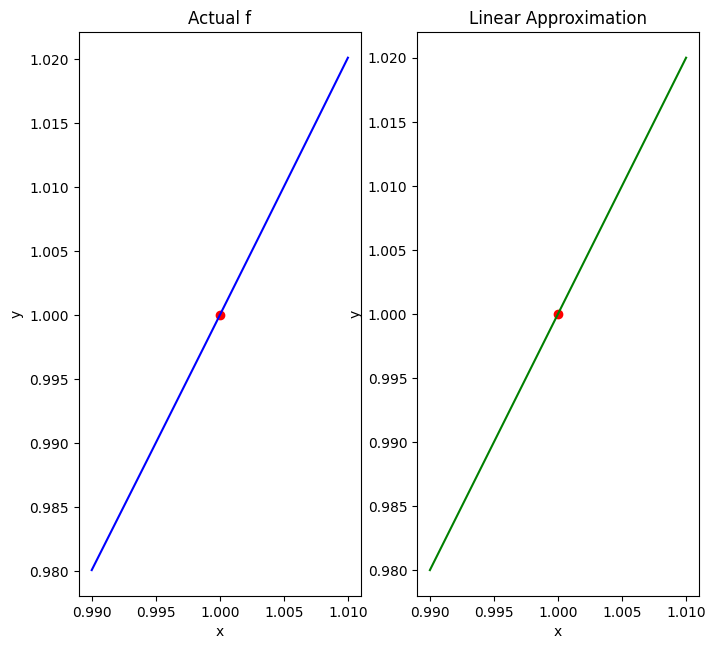
\includegraphics[width= 12cm]{./figures/6.8a.png}
    \end{center}
    which stretches twice in $y$ as it does in $x$.

    \textbf{(b)}
    \[
    Jf_{(0, 0)} = \begin{pmatrix}
    e^{2x^2 + 2x + y} (4x + 2) & e^{2x^2 + 2x + y} \\
    3 \cos (3x) + \sin(x +y) & \sin(x+y)
    \end{pmatrix}_{(x, y) = (0, 0)} = \begin{pmatrix}
        2 & 1 \\
        3 & 0
    \end{pmatrix}
    \]
    
    Its singular values are $\sqrt{2\sqrt{10} + 7} \approx 3.65, \sqrt{7 - 2\sqrt{10}} \approx 0.82$.

    And $3.65/0.82 \approx 4.44$
    \begin{center}
        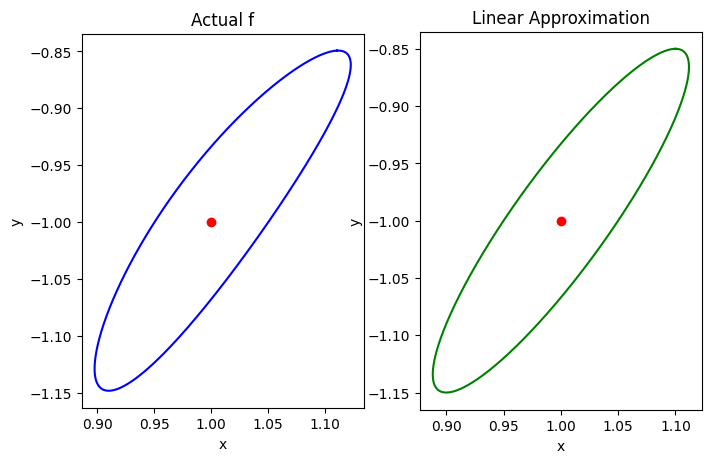
\includegraphics[width= 12cm]{./figures/6.8b.png}
    \end{center}

    \textbf{(c)}
    \[
    Jf_{(1, 1)} = \begin{pmatrix}
    2x & 1\\
    2y & 2x \\
    -1 & 3/y
    \end{pmatrix}_{(x, y) = (1, 1)} = \begin{pmatrix}
    2 & 1 \\
    2 & 2 \\
    -1 & 3
    \end{pmatrix}
    \]

    Its singular values are $\frac{\sqrt{2} \sqrt{\sqrt{61} + 23}}{2} \approx 3.92, \frac{\sqrt{2}\sqrt{23 - \sqrt{61}}}{2} \approx 2.75$.
    $3.92/2.75 \approx 1.42$
    \begin{center}
        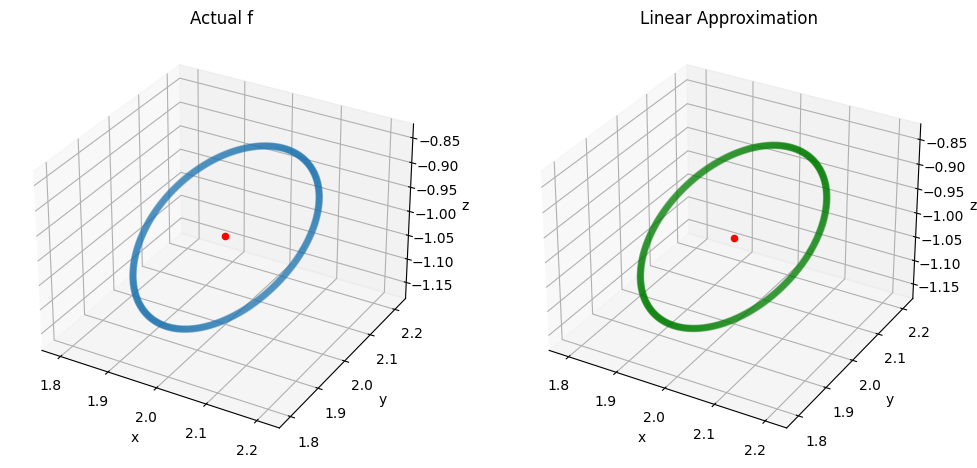
\includegraphics[width= 12cm]{./figures/6.8c.png}
    \end{center}

    \textbf{(d)}
    \[
    Jf_{(0, 0, 0)} = \begin{pmatrix}
        1 + y\cos(xy) & 1 + x\cos(xy) & 0\\
        0 & 1 & 1 \\
        1 & 1 & 1
    \end{pmatrix}_{(x, y, z) = (0, 0, 0)} = \begin{pmatrix}
    1 & 1 & 0 \\
    0 & 1 & 1\\
    1 & 1 & 1
    \end{pmatrix}
    \]
    Its singular values are $\sqrt{2\sqrt{2} + 3} \approx 2.41, 1, \sqrt{3 - 2\sqrt{2}} \approx 0.41$.
    \begin{center}
        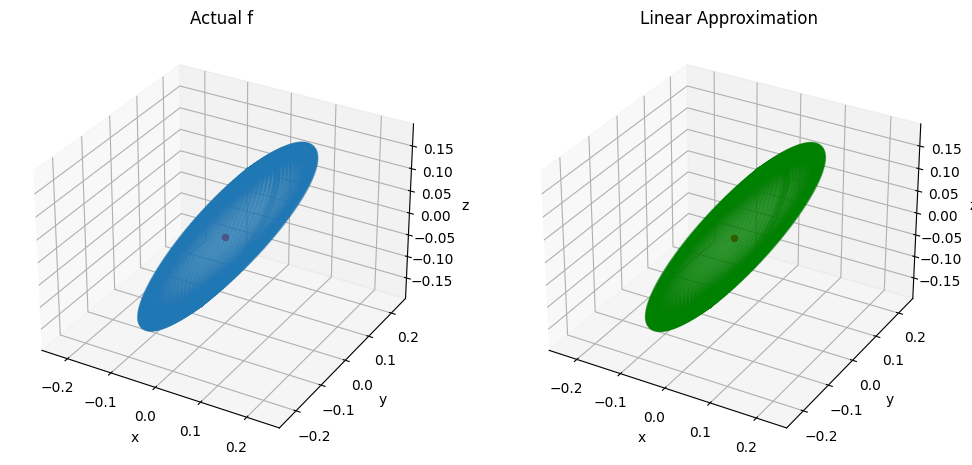
\includegraphics[width= 12cm]{./figures/6.8d.png}
    \end{center}
\end{solution}

\begin{problem} [IV \redtext{done}]
Let $U \subset \bbr^n$, and let $f: U \to \bbr$ be a function. For $v, w \in \bbr^n$ (viewed as $n \times 1$ matrices), denote by $\iprod{v}{w} = v \cdot w = v^tw$ the standard Euclidean dot product. Recall that $|v| = \iprod{v}{v}^{1/2}$.
\begin{enumerate} [(a)]
    \item Suppose that $f$ is differentiable at $p \in U$, with derivative $Df_p \in \call(\bbr^n, \bbr)$. Show that there is a unique vector $w \in \bbr^n$ such that, for all $v \in \bbr^n$: \[
              \iprod{v}{w} = Df_p(v).
          \]
          The vector $w$ is called the gradient vector of $f$ at $p$ and is denoted $grad_p(f)$.
    \item Show that, with respect to the standard basis $e_1, \dots, e_n$ of $\bbr^n$, we have \[
              grad_p(f) = \begin{pmatrix}
                  \frac{\partial f}{\partial x_1} \\
                  \frac{\partial f}{\partial x_2} \\
                  \dots                           \\
                  \frac{\partial f}{\partial x_n}
              \end{pmatrix}
          \]
    \item Show that $\norm{Df_p} = \abs{grad_p(f)}$, and that the maximum value of the function $g: S^{n-1} \to \bbr$ on the $(n-1)-$sphere defined by \[
              g(v) = Df_p(v)
          \]
          is attained at $v = grad_p(f)/\abs{grad_p(f)}$. Thus the direction of the gradient vector field $f(p) = grad_p(f)$ is the direction of steepest ascent (increase) for the function $f$, and the magnitude $|f(p)|$ is the greatest (to first order) rate of increase of the function $f$ at $p$.
    \item Show that if $\gamma: (-\epsilon , \epsilon) \to U$ is a differentiable curve through $p$ along which $f$ is constant (i.e. if $\gamma (0) = p$ and $f(\gamma(t)) = f(\gamma(0))$ for all $t \in (-\epsilon, \epsilon)$), then $\gamma'(0)$ is perpendicular to $grad_p(f)$; i.e. \[
              \iprod{grad_p(f)}{\gamma'(0)} = 0.
          \]
          In words, this means that the gradient of $f$ is everywhere perpendicular to the level sets $f^{-1}(c), c \in \bbr$ of $f$.
    \item For the function $f(x, y) = \sin(2x+y) + e^{\cos(xy)}$, plot, using a computer program, the graph of the function $f$ (in 3D), and the level sets of $f$ in the region $[-2, 2] \times [-2, 2]$. Then plot the gradient vector field for $f$. Wolfram alpha works, for example. Think about steepest ascent in terms of climbing the graph and level sets in terms of walking at a fixed elevation on the graph. The graph of the level sets is like a map of the mountain, and the gradient vector field points at the shortest, most exhausting, path up. You don't have to write down your thoughts, but do supply pics of the graphs.

    \item *Explain how to generalize this notion of gradient to any inner product on $\bbr^m$. In this way, one can use a different measure of increase of the function (if you're a budding economist or physicist, this could be useful...). The notion of gradient generalizes even more: you can let the inner product $\iprod{\cdot}{\cdot}_p$ depend on the point $p$! (This is the beginning of Riemannian geometry).
\end{enumerate}

\end{problem}
\begin{solution}
    \textbf{(a)} $f$ is differentiable at $p \in U$, let $J$ be the Jacobian matrix of $Df_p$, using the standard basis of $\bbr^n$ and $\bbr$. $J$ is a $1 \times n$ matrix, $J \in \calm_{1 \times n}$.

    We want to show that $w = J^t \in \calm_{n \times 1}$, or alternatively $\in (\bbr^n)$ satisfies $\iprod{v}{w} = Df_p(v)$. Indeed, \[
        \iprod{v}{w} = w^t v = J v = Df_p(v) \forall v \in U
    \]
    and we're done.

    To prove uniqueness, suppose there exists $w_1, w_2$ that satisfy \[
        \iprod{v}{w_1} = \iprod{v}{w_2} = Df_p(v) \forall v \in U
    \]
    then \[
        T_1(v) = T_2(v) = Df_p(v) \forall v \in U
    \]
    where $T_1, T_2$ are linear transformations $U \to \bbr$ that has $w_1^t$ and $w_2^t$ respectively as their Jacobian matrices. Therefore $T_1$ and $T_2$ are linear transformations that satisfy the properties of the total derivative of $f$. But $Df_p$ is the unique linear transformation that satisfies those properties, so $T_1 \equiv T_2 \equiv Df_p \implies w_1 = w_2$. \qed

    \textbf{(b)} Since \[
        J = \begin{pmatrix}
            \frac{\partial p }{\partial x_1} & \frac{\partial p }{\partial x_2} & \cdots & \frac{\partial p }{\partial x_n}
        \end{pmatrix}
    \]
    and we've shown above that \[
        grad_p(f) = J^t = \begin{pmatrix}
            \frac{\partial p }{\partial x_1} \\
            \frac{\partial p }{\partial x_2} \\
            \dots                            \\
            \frac{\partial p }{\partial x_3} \\
        \end{pmatrix} \qed
    \]

    \textbf{(c)} Let $v \in \bbr^n$. Then using Cauchy-Schwarz: \[
        \abs{Df_p(v)} = \abs{\iprod{J^t}{v}} \leq \abs{J^t}\abs{v} = \abs{grad_p(f)}\abs{v} \implies \frac{\abs{Df_p(v)}}{\abs{v}} \leq \abs{grad_p(f)}
    \]
    with equality achievable when $v$ and $grad_p(f)$ are linearly dependent, meaning \[
        v = \lambda grad_p(f)
    \]
    for some $\lambda \in \bbr$.

    Therefore \[
        \norm{Df_p} = \sup_{v \in \bbr^n, v \neq 0} \left\{\frac{|Df_p(v)|}{|v|}\right\} = \abs{grad_p(f)}
    \]
    since the max is achieved in $\bbr^n$.

    Furthermore, with $g$ defined for $v \in S^{n-1}$:\[
        g(v) = Df_p(v)
    \]
    The maximum, as aforementioned, is achieved when  \[
        v = \lambda grad_p(f)
    \]
    Find $\lambda$:
    \[
        |v| = \lambda |grad_p(f)| \implies \lambda = 1/|grad_p(f)|
    \]
    so the max is achieved when \[
        v = \lambda grad_p(f) = grad_p(f) / |grad_p(f)|
    \]
    as required. \qed

    \textbf{(d)} What we WTS is equivalent to:\[
        \iprod{grad_p(f)}{\gamma'(0)} = 0 \Leftrightarrow J(\gamma'(0)) = 0 \Leftrightarrow Df_p(\gamma'(0)) = 0
    \]
    Since $f$ is differentiable at $p$:
    \[
        f(\gamma(t)) = (f(p)) + Df_p(\gamma(t) - p) + R(\gamma(t) - p)
    \]
    where \[
        \lim_{\gamma(t) \to p} \frac{\abs{R(\gamma (t) - p)}}{\abs{\gamma(t) - p}} = 0
    \]

    Then:
    \begin{equation} \label{eq1}
        \frac{1}{t} Df_p(\gamma(t) - p) + \frac{1}{t}R(\gamma(t) - p) = \frac{1}{t} [f(\gamma(t)) - f(p)]  = 0
    \end{equation}
    We try to take the limit as $t \to 0$.

    1. Since $\gamma$ is differentiable, \[
        \gamma(t) = \gamma(0) + D\gamma_{0}(t) + R(t)
    \]
    which implies \[
        \lim_{t \to 0}\left(\frac{\abs{\gamma(t) - \gamma(0)}}{|t|}\right) = \lim_{t \to 0}\left(\frac{\abs{D \gamma_0(t) + R(t)}}{|t|}\right)
    \]
    which is squeezed:
    \[
        \lim_{t \to 0}\left(\frac{\abs{D \gamma_0(t)} - \abs{R(t)}}{|t|}\right) \leq \lim_{t \to 0}\left(\frac{\abs{D \gamma_0(t) + R(t)}}{|t|}\right) \leq\lim_{t \to 0}\left(\frac{\abs{D \gamma_0(t)} + \abs{R(t)}}{|t|}\right)
    \]
    therefore \begin{equation} \label{eq2}
        |D\gamma_0(1)| \leq \lim_{t \to 0}\left(\frac{\abs{D \gamma_0(t)} - \abs{R(t)}}{t}\right) \leq |D\gamma_0(1)|
    \end{equation}
    so the limit evaluates to $M = |D\gamma_0(1)| \in \bbr$.

    2. Since $\gamma$ is differentiable, and therefore continuous at 0, $t \to 0 \implies \gamma(t) \to p$. Therefore \begin{equation} \label{eq3}
        \lim_{t \to 0} \frac{|R(\gamma(t) - p)|}{|\gamma(t) - p|} = \lim_{\gamma(t) - p} \frac{|R(\gamma(t) - p)}{|\gamma(t) - p|} = 0
    \end{equation}

    From \eqref{eq2} and \eqref{eq3}, the following limit exists: \[
        \lim_{t \to 0}\frac{|R(\gamma(t) - p)|}{|t|} = \left(\lim_{t \to 0} \frac{|R(\gamma(t) - p)|}{|\gamma(t) - p|}\right) \left( \lim_{t \to 0}\frac{|\gamma(t) - p|}{|t|}\right) = 0M = 0
    \]
    which implies \[
        \lim_{t \to 0}\frac{R(\gamma(t) - p)}{t} = 0
    \]
    Therefore, taking $t \to 0$ in \eqref{eq1}, we have:
    \begin{align*}
        0 & = \lim_{t \to 0} \frac{Df_p(\gamma(t) - p)}{t}                                                                 \\
          & = Df_p\left(\lim_{t \to 0} \frac{\gamma(t) - \gamma(0)}{t}\right) \:\text{(since $Df_p, \gamma$ continuous)}\: \\
          & = Df_p(\gamma'(0))
    \end{align*}

    \textbf{(e)}
    \begin{center}
        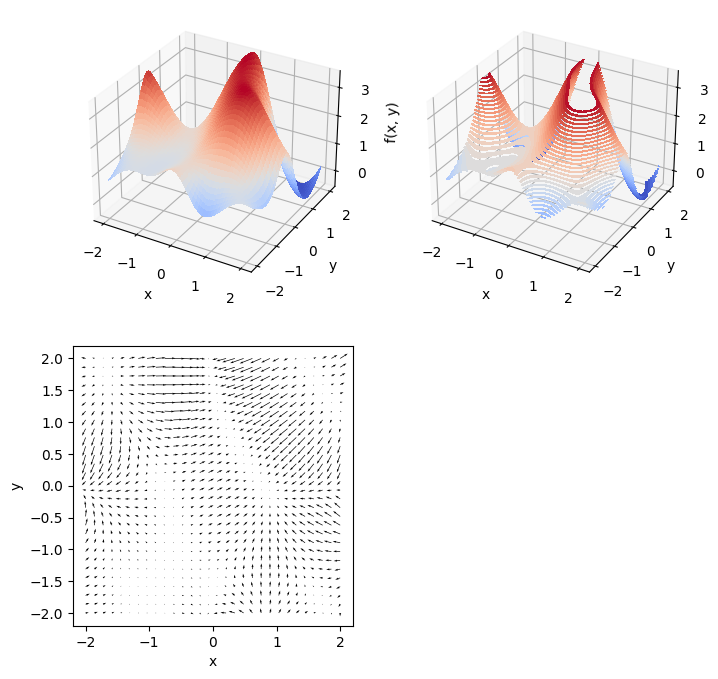
\includegraphics[width = 15cm]{./figures/6.9e.png}
    \end{center}

    \textbf{(f)} To generalize this notion of gradient to any inner product on $\bbr^m$, e.g., $\iprod{\cdot}{\cdot}_p$, to find $grad_p(f)$ at each point $p$, we first find the level curve of $f$ that goes through $f(p)$, i.e., the curve $\gamma: (-\epsilon , \epsilon) \to U$ such that $f(\gamma(t)) = f(\gamma(0)) = f(p)$.

    Then $grad_p(f) \in U$ can be defined as the vector that is perpendicular to $\gamma'(0)$, i.e. \[
        \iprod{grad_p(f)}{\gamma'(0)} = 0
    \]
\end{solution}
\end{document}